% Figura Anexo II: el modelo de Cagan: (a) demanda de saldos reales; (b) impuesto inflacionario (señoreaje)
\documentclass[tikz,border=3pt]{standalone}
\usepackage[T1]{fontenc}
\usepackage[utf8]{inputenc}
\usetikzlibrary{arrows.meta,calc,positioning}
\begin{document}
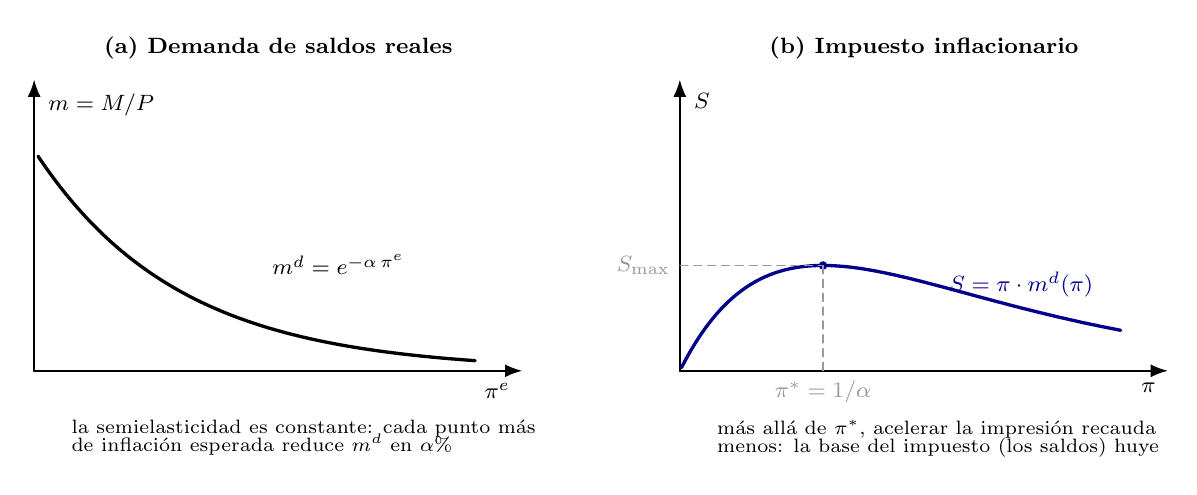
\begin{tikzpicture}[>={Latex[length=2.2mm]}, line cap=round, font=\footnotesize,
  eje/.style={->, thick},
  curva/.style={very thick},
  nueva/.style={very thick, blue!55!black},
  guia/.style={densely dashed, gray!80},
  pto/.style={circle, fill=black, inner sep=1.1pt}]
  % ---------- Panel (a): demanda de saldos reales ----------
  \node[font=\footnotesize\bfseries] at (3.1,4.1) {(a) Demanda de saldos reales};
  \draw[eje] (0,0) -- (6.2,0) node[below left=1pt]{$\pi^{e}$};
  \draw[eje] (0,0) -- (0,3.7) node[below right=2pt]{$m=M/P$};
  \draw[curva, domain=0.05:5.6, samples=80] plot (\x,{2.8*exp(-0.55*\x)});
  \node[anchor=west] at (2.9,1.35) {$m^{d}=e^{-\alpha\,\pi^{e}}$};
  \node[align=left, anchor=north west] at (0.35,-0.5) {\scriptsize la semielasticidad es constante: cada punto más\\[-3pt]\scriptsize de inflación esperada reduce $m^{d}$ en $\alpha\%$};
  % ---------- Panel (b): señoreaje ----------
  \begin{scope}[xshift=8.2cm]
    \node[font=\footnotesize\bfseries] at (3.1,4.1) {(b) Impuesto inflacionario};
    \draw[eje] (0,0) -- (6.2,0) node[below left=1pt]{$\pi$};
    \draw[eje] (0,0) -- (0,3.7) node[below right=2pt]{$S$};
    \draw[nueva, domain=0.02:5.6, samples=90] plot (\x,{2*\x*exp(-0.55*\x)});
    \node[anchor=west, blue!55!black] at (3.3,1.1) {$S=\pi\cdot m^{d}(\pi)$};
    \node[pto, fill=blue!55!black] (Smax) at (1.818,1.337) {};
    \draw[guia] (1.818,1.337) -- (1.818,0) node[below]{$\pi^{*}=1/\alpha$};
    \draw[guia] (0,1.337) node[left]{$S_{\max}$} -- (1.818,1.337);
    \node[align=left, anchor=north west] at (0.35,-0.5) {\scriptsize más allá de $\pi^{*}$, acelerar la impresión recauda\\[-3pt]\scriptsize menos: la base del impuesto (los saldos) huye};
  \end{scope}
\end{tikzpicture}
\end{document}
